\documentclass{article}

\usepackage[utf8]{inputenc}
\usepackage[T1]{fontenc}
\usepackage{amsmath}
\usepackage{xcolor} % Add this package for \textcolor
\usepackage{fancyhdr} % Add this package
\usepackage{ulem} % Add this package for better underlining
\usepackage{listings} % Add this package for code listings
\lstset{breaklines=true} % Enable line breaking in listings
\usepackage{graphicx} % Add this package for including images

\title{Documentations}
\author{Prosenjit Mondol}
\date{\today}


\pagestyle{fancy} % Enable fancy header
\fancyhead[L]{My Personal Documentations} % Left side header with documentation name
\fancyhead[C]{} % Center header empty
\fancyhead[R]{Prosenjit} % Right side header empty
\renewcommand{\headrulewidth}{1pt} % Add a horizontal line under the header



\begin{document}

\maketitle

\newpage % Start a new page after the title

\section{Data Preprocessing}
\begin{itemize}
    \item \textbf{\textcolor{blue}{\dotuline{Sampling}}}\\
        Sampling techniques are used to select a representative subset of data from a large population to reduce the computational complexity and improve the efficiency of the analysis.
    \item \textbf{\textcolor{blue}{\dotuline{Transformation}}}\\
    Transformation techniques involve manipulating raw data to create a single input, such as scaling, normalization, or encoding categorical data.
    \item \textbf{\textcolor{blue}{\dotuline{Denoising}}}\\
    Denoising techniques remove unwanted noise from the data that can lead to inaccurate results.
    \item \textbf{\textcolor{blue}{\dotuline{Imputation}}}\\
    Imputation techniques are used to fill in missing values in the data using statistical methods.
    \item \textbf{\textcolor{blue}{\dotuline{Feature extraction}}}\\
    Feature extraction techniques help to identify and extract relevant features from the data that are significant in a particular context.
    \item \textbf{\textcolor{blue}{\dotuline{Normalization}}}\\
    Normalization techniques are used to organize data for more efficient access and processing.

\end{itemize}

\section{Handle Categorical Data}

Categorical data is a type of data that represents qualitative or nominal characteristics, such as gender, occupation, Categorical data cannot be measured or compared using mathematical operations like addition or subtraction.
\subsection{Different Encoding Methods for Categorical Data}
\begin{itemize}
    \item \textbf{\textcolor{blue}{\dotuline{One-Hot Encoding}}}\\
    One-Hot Encoding creates a new binary column for each category.
    
    \item \textbf{\textcolor{blue}{\dotuline{Label Encoding}}}\\
    Label Encoding assigns a numerical value to each category.
    \begin{center}
        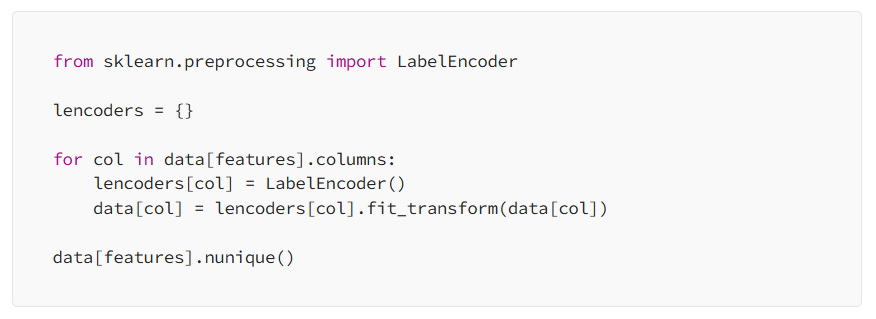
\includegraphics[width=0.5\textwidth]{label encoding} % Replace 'example-image' with your image filename (without extension)
    \end{center}
    \item \textbf{\textcolor{blue}{\dotuline{Binary Encoding}}}\\
    Binary Encoding creates new columns representing each category.
\end{itemize}


\end{document}
